\section{Background}\label{s:background}

%-------------------------------------------------------------------------
\subsection{Fragmentation}\label{ss:fragmentation}

\begin{comment}
As shown in Figure~\ref{fig:fragmentation}, filesystem fragmentation occurs when a file is stored in non-contiguous spaces on the storage medium.
This may happens even there is enough available free space in small fragments.
In the era of HDDs, the main cause of performance degradation due to file fragmentation is seek time and rotational latency.
In HDDs, there is a need for seek time to move the disk head to the track where the requested sector is located, as well as rotational latency to find it on that track.
Fragmentation increases the overhead by requiring the disk head to move more frequently, particularly having a pronounced negative impact on read operations.

\noindent {\textbf{Filesystem Fragmentation in SSDs.}}%
In flash memory, there is no seek time or rotational latency, so early researchers generally argued that SSD performance is not affected by filesystem fragmentation.
Therefore, techniques like defragmentation were thought to have only negative impacts by reducing the lifespan of flash memory due to additional write operations~\cite{defrag-mobile:atc17,fragpicker:sosp21,defrag-lfs:apsys16,no-afraid:fast24,parallel-defrag:sac22,Defragmentation_read_collision}.
However, more recent studies have shown that filesystem aging and resultant fragmentation can also lead to performance degradation in SSDs~\cite{Problem_in_SSD_Empirical,senescence:fast17,Problem_in_SSD_Mobile_Devices,survey:ictc23}.

The first reason for this is request fragmentation.
In the Linux I/O stack, a single I/O request can only represent contiguous LBA (Logical Block Address).
Fragmentation influences the non-contiguous storage of data, causing a single I/O request to be divided into multiple smaller I/O requests.\cite{IO}
This increases the total number of I/O requests, and all requests derived from a single I/O must be completed before the next process can proceed, leading to issues in I/O performance.
If multiple I/O requests are necessary for one file, the system must generate bio structures, request structures, and I/O commands corresponding to the number of requests.
This process incurs overhead in I/O request management.

Secondly, SSDs enhance read performance through prefetching, which loads subsequent data in advance based on LBA.
Fragmentation can cause this prefetching to load unnecessary data.\cite{Defragmentation_Log_write_is_ssd_to_bad} For these reasons, filesystem fragmentation is also a concern in SSDs.

\noindent {\textbf{Logical fragmentation and physical fragmentation.}}
I/O performance in flash storage is affected in different ways by logical fragmentation and physical fragmentation.\cite{janusd:atc17}
Logical fragmentation occurs when files are allocated in multiple fragmented storage spaces (extents) within the filesystem.
When a file is not stored contiguously and is spread across various locations, the filesystem recognizes this as being in a logically fragmented state.
As a result, more I/O requests are needed to read the file, which increases overhead in I/O scheduling and handshaking processes.

On the other hand, physical fragmentation happens when the data of a file is allocated non-contiguously at the physical locations of the storage device.
In flash storage, data can be distributed across multiple channels, which directly impacts I/O parallelism.
This can lead to a degradation in I/O performance.
Even if the Physical Block Address (PBA) is contiguous, if the Logical Block Address (LBA) is non-contiguous, separate I/O requests become necessary.
This increases the number of I/O requests, which can lower the overall performance of the system.
Therefore, logical fragmentation and physical fragmentation can occur independently, and appropriate measures are needed to address each issue.
\end{comment}

% Intro
Fragmentation in computer systems refers to the condition in which free space or data is scattered across non-contiguous locations.
Fragmentation can be categorized into two primary types: \emph{free space fragmentation} and \emph{data fragmentation}.


\begin{figure*}[t]
\centering
	\subfloat[Free space fragmentation] {%
		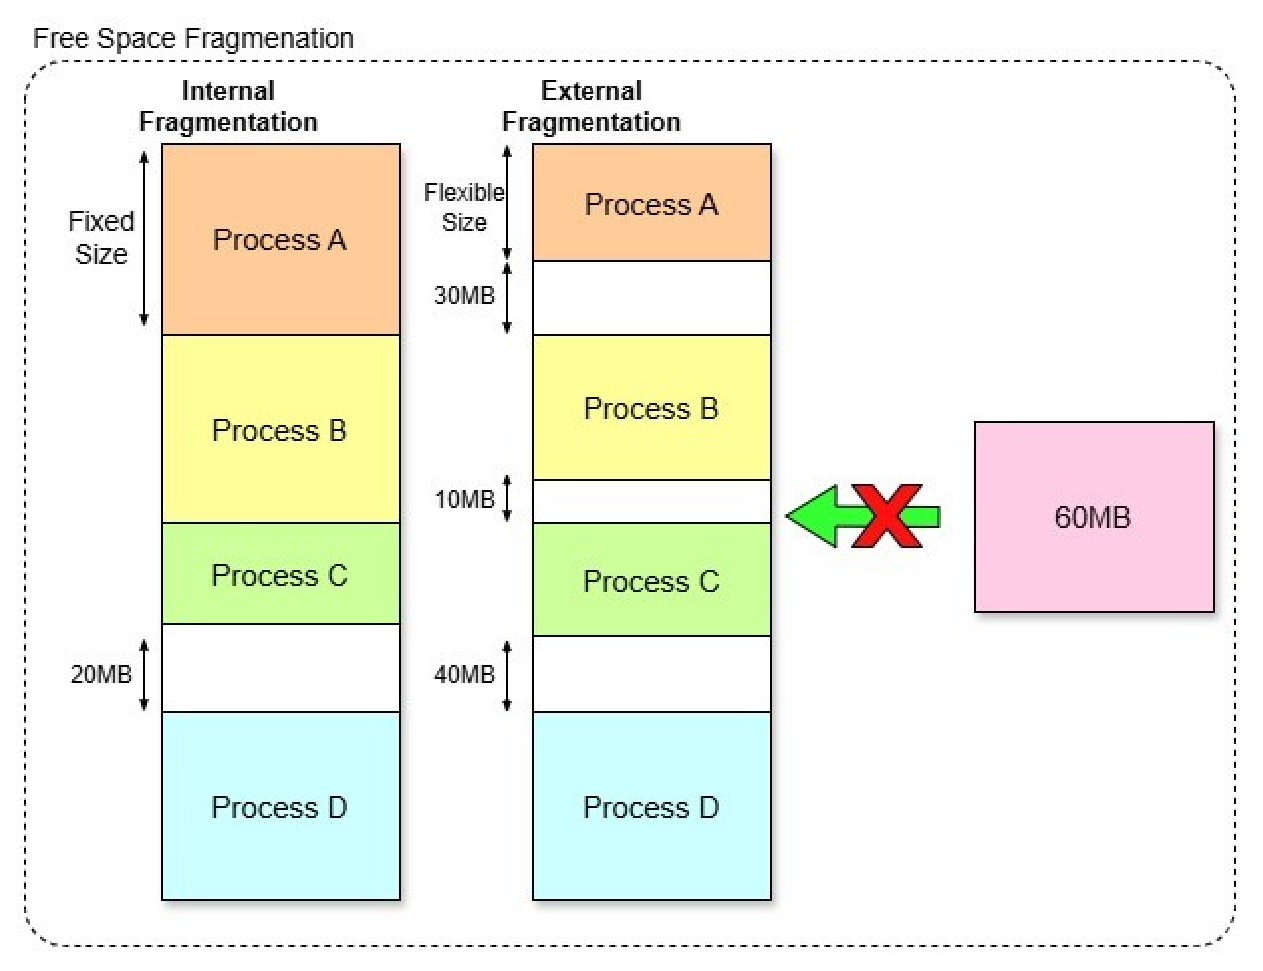
\includegraphics[height=0.25\textheight]{free-fragmentation}
		\label{f:free-fragmentation}
	}
	\hspace{0.5em}
	\subfloat[Data fragmentation] {%
		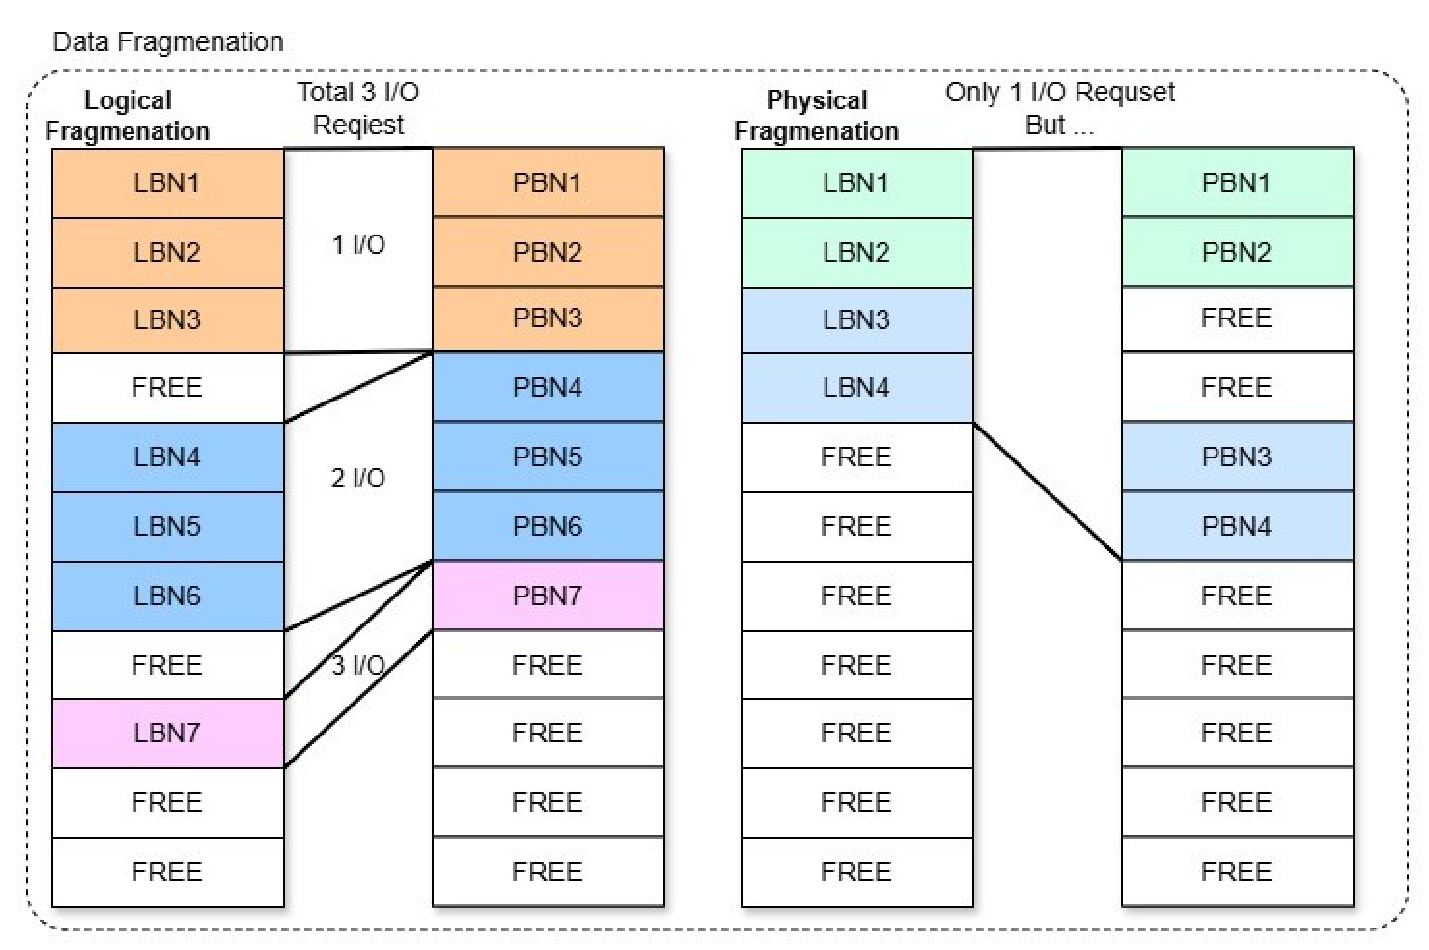
\includegraphics[height=0.25\textheight]{data-fragmentation}
		\label{f:data-fragmentation}
	}
	\caption{Types of fragmentations\label{f:fragmentation}}
\end{figure*}

% Free space fragmentation
Free space fragmentation can be further classified as internal or external fragmentation~\cite{ostep,os-textbook}.
Internal fragmentation occurs when a system employs fixed-size allocation policies, leading to allocated regions containing unused space.
In contrast, external fragmentation occurs when a system repeatedly allocates and deallocates variable-sized chunks.
Through the operations, free space is divided into into small non-contiguous fragments as illustrated in Figure~\ref{f:free-fragmentation}.
This scattered free space makes it difficult to allocate large contiguous blocks, even if the total available free space is sufficient.


% Data fragmentation
Similar to free space, data can be fragmented in computer systems.
In the context of filesystems, data fragmentation occurs when a file is stored in non-contiguous locations in a storage device.
A file may be split into multiple chunks and stored in a fragmented manner.
Notably, data fragmentation can occur even when enough contiguous space is available to store the entire file, due to prior fragmentation or allocation policies.

% Logical fragmentation
As illustrated in Figure~\ref{f:data-fragmentation}, data fragmentation can happen in two forms: \emph{logical fragmentation} and \emph{physical fragmentation}~\cite{janusd:atc17}.
Modern storage devices expose their storage space through logical block addresses~(LBAs), and the host specifies the target data for operations using a starting logical block number~(LBN) and the number of consecutive logical blocks.
Consequently, filesystems must make one I/O request per contiguous LBA chunk.
When a file is fragmented, the filesystem must generate more I/O requests than unfragmented data, thereby experiencing increased interfacing overhead.
Logical fragmentation occures primarily due to the space allocation policies of filesystems.

% Physical fragmentation
Physical fragmentation originates from the discrepancy between logical and phycal address spaces.
Modern storage devices often utilize high-density storage media with complex characteristics and inherent limitations.
Additionally, they typically employ sophisticated data paths and highly parallel architectures for delivering high performance.
As a result, the logical address space exposed to the host does not necessarily align with the physical address space on the storage media and underlying archtecutre.
Consequently, even if the host issues a single request for a logically contiguous chunk, the device may process it through multiple internal operations.
This is becoming more pronounced in recent devices, where interfacing overhead becomes a non-negligible portion of overall performance~\cite{Problem_in_SSD_Empirical,senescence:fast17,Problem_in_SSD_Mobile_Devices,survey:ictc23,no-afraid:fast24,defrag-mobile:atc17,fragpicker:sosp21}



%-------------------------------------------------------------------------
\subsection{Flash Translation Layer*}\label{ss:ftl}

\begin{comment}
Programs based on the filesystem of a typical operating system recognize disks on a sector basis.
However, in the case of SSDs, storage units are implemented based on pages and blocks.
This means that sector-based programs cannot write directly to SSDs.
Nevertheless, SSDs can easily accommodate these programs because they use the same host interface as HDDs.
To facilitate this, something is needed to assist SSDs in writing for sector-based programs, which is known as the Flash Translation Layer (FTL).

FTL performs two important functions within the SSD: Logical Block Mapping and Garbage Collection (GC).
FTL is responsible for converting logical addresses to physical address values to store logical sectors in physical pages, which is referred to as logical block mapping.
Block mapping is stored in the SSD's memory for quick access and consists of a table containing Logical Block Addresses (LBA) and Physical Block Addresses (PBA).
Additionally, SSDs cannot perform in-place updates.
Therefore, when new data arrives, existing data must be deleted before the new data can be stored.
At this time, the SSD uses GC to preemptively free up space for deleted data, which also contributes to the durability of the SSD.

In this study, we copy and store information from the SSD.
However, accessing the SSD's FTL from the outside is not feasible due to reasons such as security and complexity.
\end{comment}

% Why FTL?
Programs based on the filesystem of a typical operating system recognize disks on a sector basis.
However, flash memory, which is used for building SSDs, is organized with pages and blocks.
This means that sector-based programs cannot write directly to SSDs.
Nevertheless, SSDs can easily accommodate these programs because they use the same host interface as HDDs.
To facilitate this, 
To bridge the gap and to faciliate the managing of flash storage, something is needed to assist SSDs in writing for sector-based programs, which is known as the flash translation layer~(FTL).

% Mapping
FTL performs two important functions within the SSD: logical block mapping and garbage collection~(GC).
FTL is responsible for converting logical block addresses to physical address values to store logical sectors in physical pages, which is referred to as logical block mapping.
The mapping is stored in the SSD's flash and cached in the memory for quick access and consists of a table containing logical block addresses~(LBA) and physical block addresses~(PBA).
Additionally, SSDs cannot perform in-place updates.
Therefore, when new data arrives, existing data must be deleted before the new data can be stored.
At this time, the SSD uses GC to preemptively free up space for deleted data, which also contributes to the durability of the SSD.

% Private FTL
However, accessing the FTL of SSDs from the outside of device is usually infeasible.
SSD manufacturers make propritery designs due to reasons such as security and complexity.
Such a hidden internal of FTL results in another issues.
There have been studies to expose the internals of SSDs to the host~\cite{ocssd:fast17,zns:atc21,fdp}.
However, the details of FTL implementations and configurations are not usually publicly available.
